\newsection{Meccanismi di controllo e di rendicontazione}
\subsection{Meccanismi di controllo}
Il sistema di ticketing adottato, descritto nel documento \emph{Norme di Progetto v1.0.0}, permette di suddividere e controllare le varie attività. In particolare, è possibile visualizzare:
\begin{itemize}
\item{\textbf{Calendario attività}}: la data di fine delle varie attività è indicata in un calendario e gestita automaticamente dal sistema di ticketing;  
\item{\textbf{Dettaglio attività}}: ogni attività include diverse informazioni, quali personale incaricato, stato dell'attività e data di fine prevista. 
\end{itemize}
\subsubsection{Controllo dei ritardi}
Ogni attività, assegnata a uno o più componenti del gruppo, deve essere svolta entro una data prestabilita. In questo modo è possibile pianificare in modo chiaro ed efficace l'insieme delle varie attività. Il mancato completamento entro la data prevista comporta un ritardo. In questo caso, si è deciso di chiudere la task tenendo conto delle ore effettive di lavoro fino a quel momento. Successivamente, verrà aperta una nuova task uguale alla precedente contrassegnata da una "R", che simboleggia un ritardo nel completamento. Così facendo, le ore aggiuntive necessarie possono, in ogni caso, essere segnate nella nuova task. Alla fine, si avrà un totale delle ore impiegate, le quali verranno rendicontate.

\subsubsection{Controllo delle fasi di processo}
Il ciclo \gl{PDCA} descritto nel documento \emph{Piano di progetto v1.0.0} distingue lo stato di avanzamento di un'attività. Utilizzando il numero di attività presenti nel sistema di ticketing e un \gl{grafico ad area in pila} che rappresenta tutte le attività in determinata fase del ciclo, vengono visualizzati in quali stati le attività si trovano. \\
In questo modo si possono ricavare informazioni in  modo rapido e di particolare importanza, come:
\begin{itemize}
\item{La velocità con la quale le attività passano di stato in stato, fino al completamento della fase \emph{act}.}
\item{Eventuali periodi di stallo di una o più attività all'interno di una fase specifica.} \\ \\
\end{itemize}  
\begin{figure} [H]
	\centering
	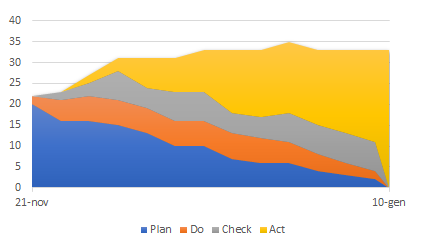
\includegraphics[scale=1]{../PianoDiProgetto/Img/Grafico_PDCA.png}
	\caption{Figura 6.2.1: Grafico ad area in pila che raffigura il ciclo PDCA}\label{}
\end{figure} 
\subsubsection{Controllo delle metriche di progetto}
Nel documento \emph{Piano di Qualifica v1.0.0} sono riportate le metriche \gl{Budget Variance (BV)} e \gl{Schedule Variance (SV)}. Grazie ad esse lo stato di avanzamento delle attività può essere controllato e quantificato e i possibili problemi di costo/schedulazione individuati prima che possano diventare critici. In particolare, attraverso le metriche Budget Variance e Schedule Variance, è possibile rispettivamente:
\begin{itemize}
\item{Verificare se le spese sono state maggiori a quanto previsto dal budget;}
\item{Verificare se un'attività è in linea, in anticipo o in ritardo rispetto alla schedulazione delle attività.}
\end{itemize}

\subsection{Meccanismi di rendicontazione}
Il sistema di ticketing adottato, descritto nel documento \emph{Norme di Progetto v1.0.0}, permette ad ogni membro di rendicontare le ore spese per una specifica attività. In particolare, è possibile visualizzare:
\begin{itemize}
\item{Ore di lavoro complessive per un attività;}
\item{Ore di lavoro complessive per un ruolo.}
\end{itemize}
\pagebreak